% !TEX root = diplomarbeit.tex
\chapter{Mechanik}

\renewcommand{\kapitelautor}{Autor: Alexander Punz}

\section{Allgemeine technische Planung}

		\subsubsection{Allgemeine Informationen über 3D Drucken}

		Die Technologie des 3D Druckens hat in den letzten Jahren immer mehr an Popularität gewonnen. Mit Hilfe des 3D Druckers kann man fast alle vorstellbaren Formen anfertigen.
		Es gibt verschiedenste Verfahren wie man ein Werkstück anfertigen kann: Laser Sintern, Stereolithographie, Drucken mit flüssigen Materialien, etc.
		In diesem Projekt wird nur die Variante des Druckens mit flüssigen Material verwendet.
		Diese ist kostengünstig \bzw genau genug für die Teile. Wie der Name schon sagt, wird Material in einem Druckkopf geschmolzen und dann Schicht für Schicht auf der Druckplatte aufgetragen.
		Der Druckkopf fährt nur in X und Y Richtung, die Höhe wird mit der Druckplatte selbst verfahren.

		Meist werden Drucker über einen Maschinencode gesteuert, dem sogenannten „G-Code“. In diesem Code werden die Punkte (Koordinaten) definiert, die der Extruder (Druckkopf) abfahren muss.
		Die folgende Abbildung zeigt ein Beispiel eines Maschinencodes.

			\begin{figure}[tbh]
			\begin{centering}
			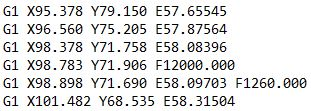
\includegraphics[width = 0.45\textwidth]{Bilder/gcode_erklaerung}
			\par\end{centering}
			\caption{Maschinencode Erklärung}
			\label{gcode_erklaerung}
			\end{figure}

			% Table generated by Excel2LaTeX from sheet 'Tabelle1'
			\begin{table}[htbp]
  		\centering
  		\caption{Befehle G Code}
	    \begin{tabular}{ll}
	    G1    & Kontrollierte Bewegung \\
	    X, Y  & Koordinaten in horizontaler und vertikaler Richtung \\
	    E     & Angabe der Menge des Filaments, dass in den Extruder geschoben werden muss \\
	    F     & Geschwindigkeit, mit der das Material in den Extruder geschoben wird (mm/min) \\
	    \end{tabular}%
	  	\label{tab:befehle gcode}%
			\end{table}%

		Je nachdem wie der Drucker aufgebaut ist, werden die Produkte genau oder nur grob angefertigt. Sehr genaue Teile kann man am besten in einem Drucker produzieren, der einen geschlossenen Druckraum \bzw eine beheizte Druckplatte hat.
		Besonders an dünnen Platten merkt man das. Wenn der Druckraum nach \bzw während des Druckvorgangs warm ist, kühlt das Werkstück an jeder Stelle fast gleich ab.
		Ist der Druckraum offen, kühlt das Werkstück in der Mitte schneller ab, kühles Material zieht sich zusammen, daher biegt sich das Material auf.

		Es kann vorkommen, dass ein Teil nur so gedruckt werden kann, wenn es nicht komplett auf der Druckplatte aufliegt zum Beispiel ein Steg, der „in der Luft“ liegt oder eine Bohrung im Werkstück, die horizontal gedruckt werden muss.
		In solchen Fällen, druckt der Drucker unter diesem Steg Stützmaterial. Basierend auf diesem Stützmaterial, wird dann die gewünschte Form gedruckt.
		Das Stützmaterial ist so gefertigt, dass man es leicht von dieser abbrechen kann, ohne dass Rückstände zurück bleiben.

		\subsubsection{Materialeigenschaften}

		\subsubsection{Von der Idee zur Anfertigung}

		Die größte Hürde an der Realisierung einer Idee ist, eine CAD Zeichnung zu erstellen. In 3D CAD Programmen wie Creo, SolidWorks, etc. kann man ein Teil konstruieren und dann als STL (Standard Triangulation Language) File abspeichern.
		Dieses Format gibt dann nur mehr Informationen über die Oberfläche und Struktur an (siehe Abbildung \ref{stl_file_optionen}).
		Die Sehnenhöhe gibt an wie genau die Oberfläche gedruckt werden muss, die Winkelsteuerung gibt die Genauigkeit der Radien und Kanten des Teiles an.


			\begin{figure}[tbh]
			\begin{centering}
			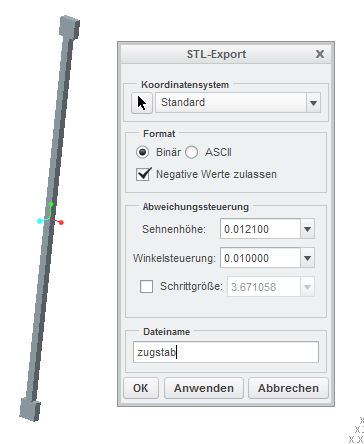
\includegraphics[width = 0.5\textwidth]{Bilder/stl_file_optionen}
			\par\end{centering}
	 		\caption{Einstellung für STL File}
			\label{stl_file_optionen}
			\end{figure}

		Mit diesem File kann man anschließend in Programmen wie Slic3r den gewünschten Maschinencode generieren lassen.
		In diesen Programmen gibt man die Lage des Werkstückes an \bzw in genaueren Einstellungen auch die Temperatur des Druckbettes, den Geschwindigkeiten und ähnliche Konfigurationen.

		Am häufigsten haben die Drucker eine USB Schnittstelle, \bzw verfügen über einen SD Karten Slot.
		Der Maschinencode wird auf diesen Speichermedien gespeichert und einfach auf den Drucker überspielt.

				\newpage


\section{Halterung für Cupcakes}

		\subsection{Technische Planung}

		Die Diplomarbeit hat sich speziell auf den Transport von Cupcakes spezialisiert, um diesen sicher transportieren zu können, ist es notwendig eine Halterung zu konzipieren.
		Zu beachten ist, dass die Halterung möglichst wenig wiegt \bzw leicht zu montieren ist.

		Der Akku wurde an der Unterseite des Hexacopters befestigt, daher war es nur mehr möglich die Halterung an der oberen Centerplate zu platzieren.
		Damit der Multicopter möglichst ausgewogen ist, muss sich das zu transportierende Objekt in der Mitte befinden.
		Die Idee war es daher, den Cupcake mit einer Halterung zu umranden, um ihn gegen Verrutsche zu sichern. Die Geometrie der Platte \bzw die Größe des Objektes hat die Befestigungsmöglichkeiten etwas eingeschränkt (siehe Abbildung \ref{platte_cupcake}).
		Die innere Reihe der Langlöcher würde sich optimal anbieten, um die Halterung befestigen zu können, die Cupcakeform kann so direkt von einer Haltevorrichtung gestützt werden.


			\begin{figure}[tbh]
			\begin{centering}
			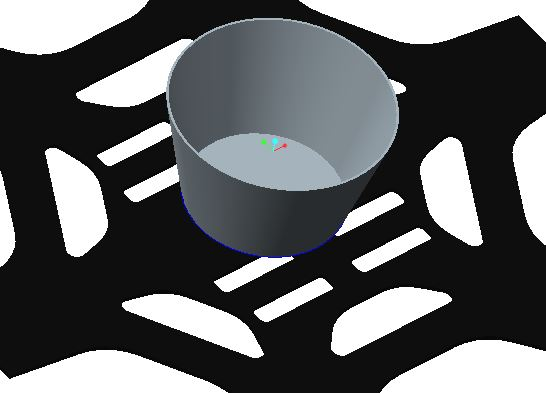
\includegraphics[width = 0.5\textwidth]{Bilder/platte_cupcake}
			\par\end{centering}
			\caption{Position Cupcake}
			\label{platte_cupcake}
			\end{figure}

	\subsection{Umsetzung}

	Wie schon in der technischen Planung erwähnt wurde, sollte der Cupcake von einer Haltevorrichtung umrandet werden.
	Die inneren Ausnehmungen der oberen Centerplate haben sich optimal angeboten, da diese direkt bis zur Form reichen.

	Es wurden Stützen konstruiert, die in den Ausnehmungen fixiert werden können und sich direkt an das Dessert anpassen.
	Die folgenden Abbildungen zeigen die konstruierten Halterungsstutzen und deren Befestigung.

			\begin{figure}[H]
			  \begin{centering}
			    \subfigure[Halterung Cupcake oben\label{halterung_cupcake_oben_grosz}]{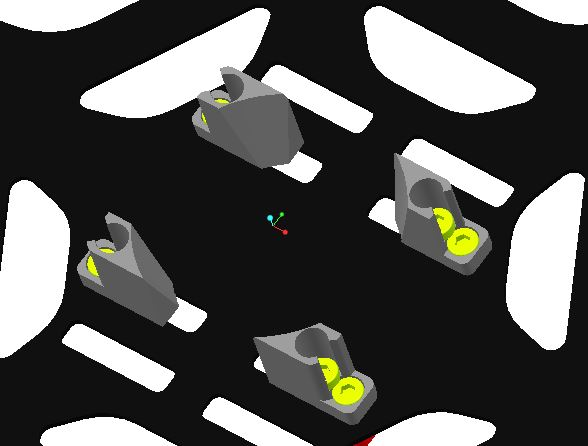
\includegraphics[width = 0.4\textwidth]{Bilder/halterung_cupcake_oben_grosz}}
			    \subfigure[Halterung Cupcake unten\label{halterung_cupcake_unten_grosz}]{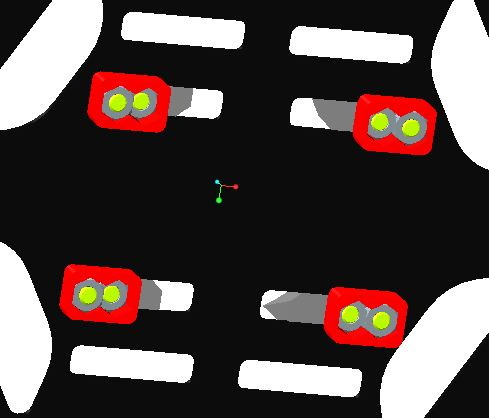
\includegraphics[width = 0.4\textwidth]{Bilder/halterung_cupcake_unten_grosz}}
			  \par\end{centering}
			  \caption{Halterung Cupcake}
			  \label{Halterung_Cupcake}
			\end{figure}

	Die Stützen (siehe Abbildung \ref{halterung_cupcake_oben_grosz}) wurden so entworfen, dass sie sich dem Radius \bzw der Höhe der Form des Cupcake anpassen.
	Die Höhe der Halterung wurde so gewählt, dass etwa die Hälfte der Cupcakeform frei liegt.
	Das soll vermeiden, dass man sich die Finger beim Entnehmen des Cupcakes an der Creme schmutzig macht.

	Die Halterung wird direkt an der Centerplate mit Durchgangsschrauben und Muttern festgeschraubt.
	Durch den Platzmangel mussten M4 Schrauben gewählt werden, da diese klein sind und trotzdem viel Beanspruchung aufnehmen können.
	Die Schlüsselweite einer M4 Mutter beträgt 7.0 mm, die Breite der Ausnehmung 6.5 mm, würde man die Schrauben direkt mit der Platte verschrauben, müsste man eine Beilagscheibe zwischenlegen, um eine größere Aufliegefläche für die Mutter zu erhalten.

	Es wurden spezielle Mutterhalter entworfen (siehe Abbildung \ref{halterung_cupcake_unten_grosz}), diese bezwecken zwei Funktionen:
	Einerseits muss man die Muttern während man die Halterung montiert nicht mehr festhalten und andererseits kann man die Schraubenverbindung viel fester anziehen, da man die Platte nicht mehr beschädigen kann.

	Der Platz für die Stutzen entlang der Langlöcher ist nur so kurz, dass sich die Köpfe der Schrauben und die Muttern schneiden würden.
	Um dieses Problem zu beheben, wurden Höhenunterschiede zwischen den Schrauben eingeplant.
	Das macht die Halterungsstutzen kompakter und verhindert Kollisionen.

	\subsection{Herausforderungen und Lösungen}

	Die größte Herausforderung beim Konstruieren war es, die Halterung an die Form des Cupcakes anzupassen.
	Die Halterungsstützen sollen an die Rundung \bzw den Durchmesserverlauf der Cupcakeform angepasst werden.
	Um die richtige Form der Stützen konstruieren zu können, wurde erst der Winkel der Cupcakeform mit der  folgenden Formel ermittelt:

			\begin{figure}[tbh]
			\begin{centering}
			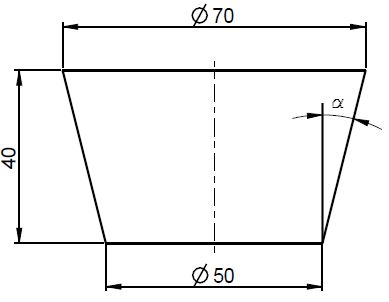
\includegraphics[width = 0.4\textwidth]{Bilder/berechnung_winkel}
			\par\end{centering}
			\caption{Berechnung des Winkels}
			\label{berechnung_winkel}
			\end{figure}

			\[
 				\tan \alpha = \frac{35mm-25mm}{40mm}  \qquad \alpha = \arctan \frac{35mm-25mm}{40mm} = \SI{14.04}{\degree}
 			\]

	Konstruiert wurde die Halterung mit einem Winkel von 15° um Ungenauigkeiten des Druckers besser kompensieren zu können.

	In der folgenden Abbildung kann man erkennen, dass manche Wände bei den Bohrungen zu dünn sind zu drucken, es entstehen dadurch Löcher.
	Dieses Problem könnte man nur lösen, wenn man die Schrauben weiter nach außen legen würde, jedoch ist das in diesem Fall nicht möglich, da die Ausnehmungen zu kurz sind.


			\begin{figure}[tbh]
			\begin{centering}
			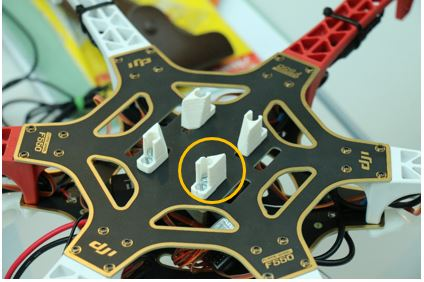
\includegraphics[width = 0.65\textwidth]{Bilder/halterung_cupcake_fertig_hinweis}
			\par\end{centering}
			\caption{Gedrucktes Halterungssystem}
			\label{halterung_cupcake_fertig_hinweis}
			\end{figure}

			\newpage

\section{Rotorschutz}

	\subsection{Technische Planung}

	In dem gewählten Bausatz des Hexacopters ist kein Rotorschutz vorhanden.
	Da der Hexacopter direkt zu den Gästen fliegen wird, ist es nicht umgänglich, den Kontakt mit den Propellern zu verhindern.
	Diese können durch die hohen Drehzahlen und die Kraft der Motoren erhebliche Verletzungen zuführen.
	Es gibt diverse Vorrichtungen für Multicopter zu kaufen, die nur die Rotorblätter schützen, jedoch keine, die auch das Eingreifen einer Hand verhindern.

	Der Rotor-, oder auch Propellerschutz genannt, soll wie ein Ring um die Rotorblätter liegen und auch auf der Ober,- und Unterseite Schutz vor Verletzungen bieten.
	Zu beachten ist jedoch auch, dass sechs Schutzvorrichtungen benötigt werden, daher sollten diese so leicht wie möglich sein, um das maximale Abfluggewicht nicht zu überschreiten.

	\subsection{Umsetzung}

	Die folgenden Abbildungen zeigen den konstruierten Propellerschutz, an dem Hexacopter montiert.

			\begin{figure}[tbh]
			\begin{centering}
			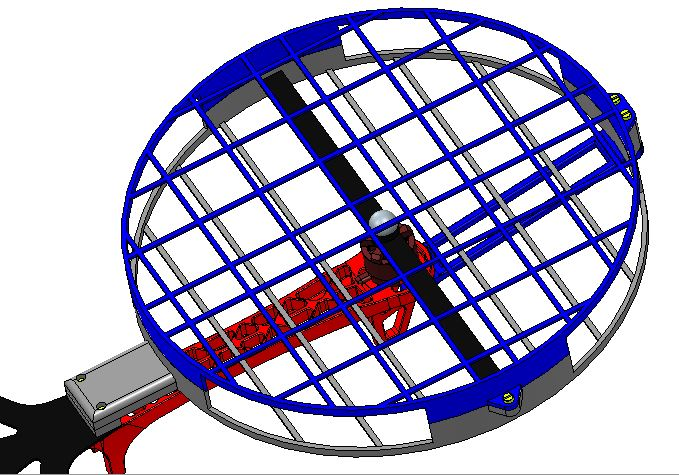
\includegraphics[width = 0.8\textwidth]{Bilder/propellerschutz_gesamt_oben}
			\par\end{centering}
			\caption{Propellerschutz oben}
			\label{propellerschutz_gesamt_oben}
			\end{figure}

			\begin{figure}[H]
			\begin{centering}
			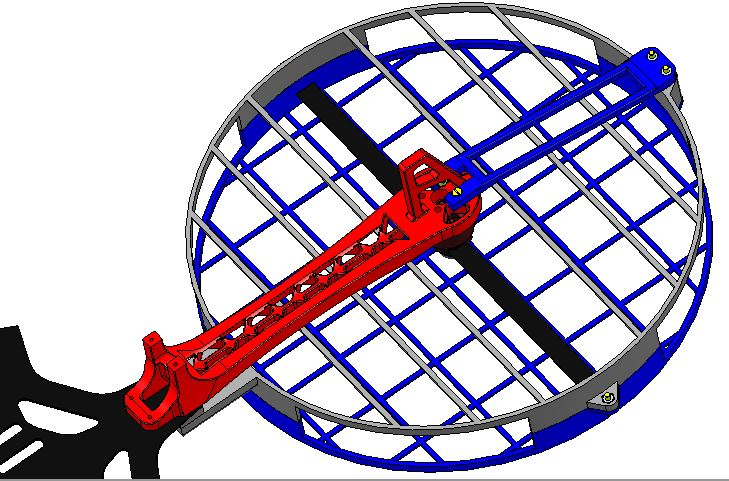
\includegraphics[width = 0.8\textwidth]{Bilder/propellerschutz_gesamt_unten}
			\par\end{centering}
			\caption{Propellerschutz unten}
			\label{propellerschutz_gesamt_unten}
			\end{figure}

	Wie geplant, umrandet der Ring das komplette Rotorblatt, im Falle eines Absturzes kann der Propeller nicht den Boden berühren und wird somit nicht beschädigt.
	Auf der Oberseite und Unterseite ist ein Gitter vorgesehen, welches Verletzungen an Personen verhindert.
	Das Gitter an der Oberseite ist etwas feiner gegliedert als an der Unterseite, da man den Cupcake von der oberen Centerplate entnehmen muss.
	An der Unterseite ist das Gitter nur gestreift konstruiert, da die Luftströmung nicht stark beeinflusst werden darf und die größere Verletzungsgefahr an der Oberseite besteht.

	Der komplette Rotorschutz wird einerseits mit zwei Schrauben am Hexacopter befestigt (siehe Abbildung \ref{propellerschutz_gesamt_oben}) und andererseits von einer Stütze (siehe Abbildung  \ref{propellerschutz_gesamt_unten},
	\textcolor{blue}{blauer Balken}) an der Unterseite gehalten. Die Stütze wird direkt an dem Motor angeschraubt, samt dem Arm des Hexacopters.
	Da die Schrauben der Centerplate und des Motors zu kurz sind, werden passende Zylinderkopfschrauben verwendet.
	Besonders bei dem Motor ist es wichtig, dass diese nicht zu lang sind, da sich der Motor nicht mehr bewegen könnte.

	Durch die Gewichtsbegrenzung \bzw der Form des Propellerschutzes, bot es sich an, diesen in einem 3D Drucker anzufertigen.
	Dazu wurde der Ring in zwei Hälften unterteilt, eine Ober,- und eine Unterseite.
	Der Ring hat einen ungefähren Innendurchmesser von 270 mm, das Druckbett eine maximale Abmessung von 270x210 mm.
	Beide Hälften mussten noch in weitere, für den Drucker passende Teile unterteilt werden.
	Die obere Hälfte wurde noch einmal in der Mitte geteilt, die Unterseite musste in vier Teile unterteilt werden (siehe folgende Abbildung \ref{propellerschutz_mitte_unterteilung}).

			\begin{figure}[tbh]
			\begin{centering}
			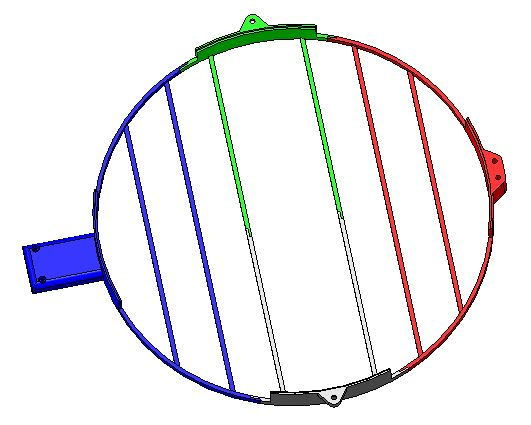
\includegraphics[width = 0.7\textwidth]{Bilder/propellerschutz_mitte_unterteilung}
			\par\end{centering}
			\caption{Propellerschutz Unterteilung}
			\label{propellerschutz_mitte_unterteilung}
			\end{figure}

			\begin{figure}[H]
			\begin{centering}
			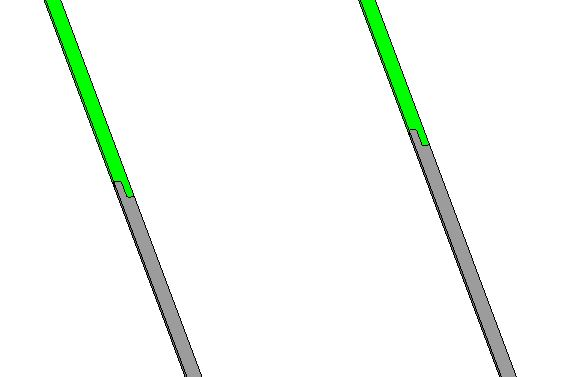
\includegraphics[width = 0.45\textwidth]{Bilder/propellerschutz_klebestellen}
			\par\end{centering}
			\caption{Propellerschutz Klebestellen}
			\label{propellerschutz_klebestellen}
			\end{figure}

	Die einzelnen Hälften  werden mit Sekundenkleber zusammengefügt, die Klebestellen wurden daher mit Nuten versehen,
	um eine größere Klebefläche zu gewährleisten (siehe Abbildung \ref{propellerschutz_klebestellen}).
	Die geklebten Hälften werden dann mit Durchgangsschrauben und Sechskantmutter miteinander verschraubt (siehe Abbildung  \ref{propellerschutz_mitte_unterteilung}),
	der kleine Absatz an der unteren Hälfte wird extra angefertigt da der Drucker kein Stützmaterial drucken müsste.

	\subsection{Herausforderungen und Lösungen}

	Eines der größten Probleme war es, den Rotorschutz so zu konstruieren, dass er stabil, aber auch sehr leicht ist.
	Im Falle eines Absturzes, würden hohe Kräfte auf den Propellerschutz wirken, daher muss dieser sehr robust gefertigt sein.
	Der Vorteil von ABS \bzw 3D Druckteilen ist, dass diese sehr elastisch sind, nicht wie Styropor zum Beispiel, es ist daher nicht notwendig den Ring dickwandig zu konstruieren.
 	Durch diesen Vorteil kann man einiges an Gewicht einsparen, das Problem besteht aber trotzdem noch darin, dass der Ring enorme Dimensionen hat.
	Eine komplette Zusammenstellung (Ring, Stütze und Schrauben) hat ein Gewicht von etwa 90 g.
	Auf sechs Propeller aufgerechnet mehr als ein halbes Kilogramm, der Hexacopter kann das zwar noch tragen, jedoch schränkt das die hardwaremäßige Erweiterung stark ein.

	Eine weitere Herausforderung war es, den Ring anzufertigen. Wie schon in dem oberen Punkt erklärt wurde, musste der Ring in sieben Teile unterteilt werden.
	Die Herausforderung lag darin, die Stücke so zu gliedern, damit sie im 3D Drucker fertigbar sind und nicht zu viel Druckzeit auf sich nehmen.
	Die Druckzeit wurde zwar schon optimiert durch die Gliederung, jedoch braucht es trotzdem noch etwa 14 Stunden alle Teile für einen Rotorschutz zu drucken.

	\subsection{Implementierung}

Die einzelnen Teile wurden wie schon erwähnt, miteinander verklebt. Bevor diese zusammengefügt wurden, musste sichergestellt werden, dass die Nuten exakt ineinander passen.
Würde dies nicht gewährleistet sein, würden die obere und untere Hälfte des Propellerschutzes nicht mehr zusammenpassen.
Die Toleranzen des Druckers, besonders bei solchen Stellen sind so groß, dass man meistens mit Feilen die Nuten nachbessern muss.
Besonders beim Verkleben der Teile ist viel Geduld nötig, da auch der Sekundenkleber nicht sofort komplett trocken ist,
es war ebenso wichtig, den richtigen Untergrund zu wählen, eine Holzplatte eignete sich am besten, da keine Rückstände blieben.

Die beiden Hälften wurden dann miteinander verschraubt, samt der Stütze.
Der gesamte Rotorschutz konnte dann mittels den vorgesehenen Schrauben an der Centerplate und dem Arm des Hexacopters befestigt werden.

			\newpage

\section{Halterung Ultraschallsensor}

	\subsection{Technische Planung}

	Die Höhe des Hexacopters wird mittels eines Ultraschallsensors gesteuert, dieser misst den Abstand von dem Boden aus.
	Damit der Sensor genaue Werte messen kann, muss er fest auf dem Multicopter befestigt werden.
	Um das gewährleisten zu können, musste eine Halterung entworfen werden, die den Ultraschallsensor optimal mit dem Hexacopter verbindet.
	Die Anforderungen an die Halterung begrenzen sich auf ein geringes Gewicht \bzw eine einfache Montagemöglichkeit.
	Der Sensor hat auf jeder Ecke eine kleine Bohrung von 1.5 mm vorgesehen, das erschwert die Befestigungsmöglichkeit des Sensors an der Halterung, da es keine gängigen Schrauben in dieser Größe gibt.

	\subsection{Umsetzung}

	Die folgende Abbildung (Abbildung \ref{halterung_ultraschall}) zeigt die CAD Konstruktion und die gefertigte (Abbildung \ref{halterung_ultraschall_fertig}) Ultraschallsensorhalterung.

			\begin{figure}[H]
				\begin{centering}
					\subfigure[CAD Konstruktion Ultraschallsensorhalterung\label{halterung_ultraschall}]{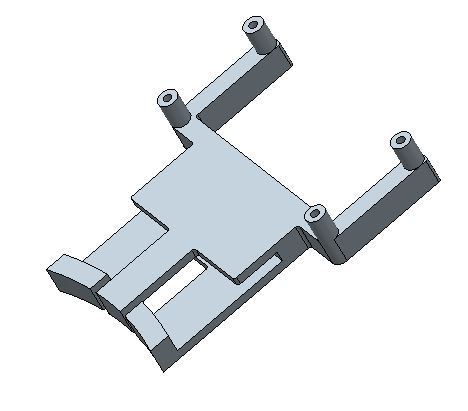
\includegraphics[width = 0.4\textwidth]{Bilder/halterung_ultraschall}}
					\subfigure[Gefertigte Ultraschallsensorhalterung\label{halterung_ultraschall_fertig}]{\includegraphics[width = 0.4\textwidth]{Bilder/halterung_ultraschall_fertig}}
				\par\end{centering}
				\caption{Ultraschallsensorhalterung}
				\label{Halterung_Ultraschallsensor}
			\end{figure}

	Das Gewicht spielte, analog zu den anderen Konstruktionen, eine wichtige Rolle.
	Materialien wie Stahl oder Aluminium wären selbst bei diesem kleinen Teil (51x46x10 mm) zu schwer geworden.
	Um das zu verhindern wurde diese Haltevorrichtung, wie auch der Propellerschutz, in einem 3D Drucker angefertigt.
	Das Teil wiegt durch die Fertigungsmethode etwa 5.5 g, das entspricht etwa dem Gewicht einer 20 Cent Münze.

	Die Halterung wird an der unteren Centerplate befestigt, da wie schon erwähnt, der Sensor von dem Boden aus misst.
	Die Befestigungsmethode ist selbst entwickelt worden, dabei handelt es sich um ein spezielles Klammersystem, welches an einer Strebe der Platte montiert werden kann (siehe Abbildung \ref{halterung_ultraschall_fertig}).
	Die Klammer besteht aus drei Stegen, auf denen jeweils ein Anschlag vorgesehen wurde.
	Die Form der Anschläge ist  exakt an die Centerplate angepasst, damit sich die Halterung so geringfügig wie möglich bewegen lässt.

	Die ideale Stärke der Stege wurde durch Versuche ermittelt, es wurde dabei das Klammersystem mit unterschiedlichen Dicken gefertigt und an dem Hexacopter getestet.
	Die optimale Stärke war deshalb wichtig, da das System nicht funktionieren würde, wenn diese falsch dimensioniert werden würde.
	Die Elastizität des Materials \bzw die gewählte Dicke der Stege ermöglicht es, diese soweit auseinanderziehen zu lassen, dass die Anschläge einfach über die Platte geschoben werden können.
	Aufgrund dieser Eigenschaften verformen sich diese auch wieder komplett zurück und fixieren somit die Halterung.

	Damit der Sensor nicht nach unten kippen kann, wurde eine Nut in die Haltevorrichtung vorgesehen.
	Droht die Halterung nach unten zu kippen, verkeilt sich diese mit der Centerplate und kann nicht mehr weitersinken.
	Die Nut ist so groß dimensioniert worden, dass sie leicht auf die Platte geschoben werden aber sich nur minimal bewegen lässt.

	Der zweite Teil der Halterung wurde so konstruiert, dass die vier Ecken der Sensorplatine gleichmäßig aufliegen können.
	Auf dem Ultraschallsensor selbst befinden sich jedoch vier Anschlussstifte, die es nicht ermöglichen, die Platine direkt auf der „Gabel“ zu befestigen.
	Um Kabel trotzdem problemlos anschließen zu können, wurde der Sensor mittels vier Stutzen 5 mm höher gelegt.

	Geplant wurde, dass der Sensor an den Stutzen mit vier Blechschrauben befestigt wird, die Durchmesser der Bohrungen sind aber so klein, dass keine gängigen Schraubendurchmesser verwendet werden können.
	Die geeigneten Schrauben werden nur in ausgewählten Geschäften verkauft, um einen viel höheren Preis \bzw längeren Lieferzeiten, als bei normalen Schrauben.
	Um den Sensor trotzdem befestigen zu können, wurden Kupferdrähte zur Fixierung verwendet.
	Da nur das Gewicht des Ultraschallsensors an den Drähten zieht, geben diese selbst bei heftigen Flugmanövern nur minimal nach.

	\subsection{Herausforderungen und Lösungen}

	Das Klammersystem hat die meiste Zeit auf sich genommen.
	Die erste Version der Halterung hat gezeigt, dass die angenommenen Dimensionen nicht umgesetzt werden konnten.
	Das Problem lag darin, dass die Halterung nicht hochkant, sondern vertikal gedruckt werden musste.
	Damit die Haltevorrichtung gedruckt werden kann, hat der Drucker Stützmaterial in die Nut gedruckt.
	Dieses Stützmaterial kann jedoch nicht restlos entfernt werden, daher musste die Höhe des Spaltes vergrößert werden.
	Es brauchte drei verschiedene Versionen der Ultraschallsensorhalterung, bis alle Parameter ideal gepasst haben, das kostete natürlich Zeit, da jedes Mal ein neues Teil gedruckt werden musste.

			\newpage

\section{Halterung PIXY CMU cam5}

	\subsection{Technische Planung}

	Der Hexacopter soll dem Gast sein gewünschtes Dessert bringen, der Weg zu dem Gast wird über Farbcodes am Boden vorgegeben.
	Um dem Farbcode folgen zu können, wird eine PIXY CMU cam5 verwendet (genaueres siehe Kapitel Sensoren).

	Die Halterung soll so konstruiert werden, dass die Kamera während des Fluges nicht wackelt, das verhindert ungenaue \bzw falsche Messwerte.
	Besonders zu beachten ist, dass die PIXY Cam immer in die Flugrichtung ausgerichtet sein muss.
	Der Flightcontroller gibt dem Hexacopter eine fixe Orientierung vor, würde die Kamera nicht in diese Richtung messen, könnte es zu Fehlmessung kommen und den Multicopter falsch navigieren.

	\subsection{Umsetzung}

	In den folgenden Abbildungen wird einerseits die konstruierte Halterung Abbildung \ref{halterung_pixy_creo})
	und andererseits die Gefertigte  mit der PIXY CMU cam5 (Abbildung \ref{halterung_pixy}).

			\begin{figure}[thb]
				\begin{centering}
					\subfigure[CAD Konstruktion PIXY Cam Halterung\label{halterung_pixy_creo}]{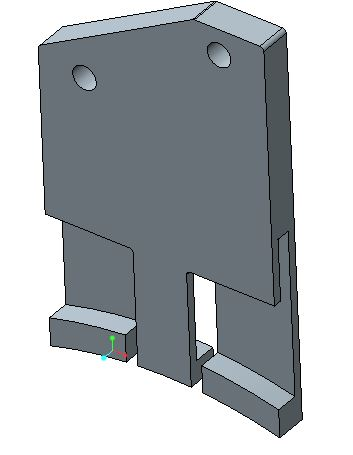
\includegraphics[width = 0.3\textwidth]{Bilder/halterung_pixy_creo}}
					\subfigure[Gefertigte PIXY Cam Halterung\label{halterung_pixy}]{\includegraphics[width = 0.4\textwidth]{Bilder/halterung_pixy}}
				\par\end{centering}
				\caption{Halterung PIXY Cam}
				\label{Halterung_PIXY}
			\end{figure}

	Aus Gewichtsgründen wurde die Halterung in einem 3D Drucker angefertigt.
	Diese wiegt etwa 5.2 g, ist also etwas leichter als die Ultraschallsensorhalterung.
	Um den Hexacopter, selbst bei so geringen Massen besser ausgleichen zu können, wurden beide Befestigungsmöglichkeiten gegenüber voneinander platziert.
	Da die PIXY Cam Halterung auf der unteren Centerplate platziert wird, konnte wieder das eigens entwickelte Klammersystem verwendet werden.
	Das garantiert auch in diesem Fall eine gute Passgenauigkeit, um den Sensor optimal zu fixieren.

	Die Kamera hat an der unteren Leiste der Platine zwei Bohrungen vorgesehen, diese wurden genutzt um den Sensor mit der Halterung zu verbinden.
	Es bot sich nicht viel Platz auf der Platine an, um den Sensor fest genug zu fixieren, jedoch reichte der untere Streifen ausreichend aus.

	Wie schon in der technischen Planung erwähnt wurde, spielt die exakte Position der PIXY Cam eine wichtige Rolle.
	Die Vorgangsweise zur Ermittlung der Ausrichtung wird mit der folgenden Abbildung erklärt.

			\begin{figure}[tbh]
			\begin{centering}
			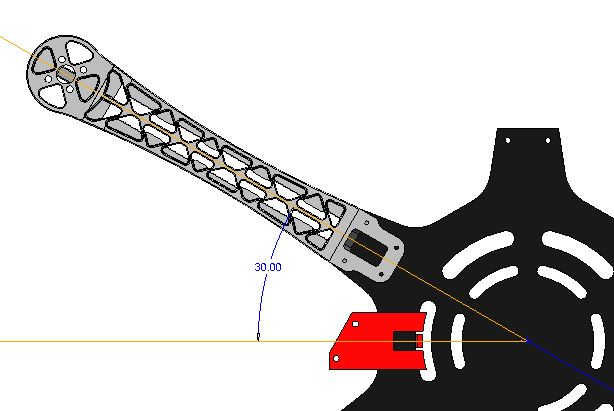
\includegraphics[width = 0.8\textwidth]{Bilder/winkel_pixy}
			\par\end{centering}
			\caption{Messung des Winkel}
			\label{winkel_pixy}
			\end{figure}

	Der Flightcontroller wurde so eingebaut, dass ein Arm des Hexacopters zur Kontrolle in die Flugrichtung steht.
	Die \textcolor{red}{Halterung} wurde genau in der Mitte der Strebe platziert, daher konnte eine Konstruktionslinie vom Mittelpunkt der Platte aus, gesetzt werden.
	Der Winkel konnte gemessen werden, indem die zweite Konstruktionslinie entlang der Mitte des Arm gesetzt wurde.
	Die Schräge ist deshalb notwendig, da der Platz auf der Platine des Sensors so begrenzt ist, dass nur die Fläche der unteren Leiste aufliegen kann.

	\subsection{Herausforderungen und Lösungen}

	Der begrenzte Platz zum Montieren der PIXY Cam an der Halterung war die größte Herausforderung.
	Das  Problem war, dass sich auf der Platine eine Kabelbuchse befindet, diese ist genau auf der Ecke des Streifens vorgesehen (siehe Abbildung \ref{pixy_back}, orange markierter Bereich).

			\begin{figure}[tbh]
			\begin{centering}
			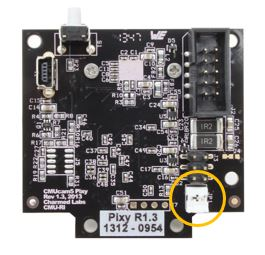
\includegraphics[width = 0.5\textwidth]{Bilder/pixy_back}
			\par\end{centering}
			\caption{PIXY Cam Hinterseite}
			\label{pixy_back}
			\end{figure}

	In den Konstruktionen wurde dieses Problem nicht behandelt, erst bei dem ersten Test hat sich gezeigt, dass die Halterung nicht komplett passt.
	Um nicht noch eine neue Version drucken und Zeit verlieren zu müssen, wurde die Kante an der linken Bohrung (siehe Abbildung \ref{halterung_pixy_creo}) passgenau mit einer Feile abgerundet.

	\subsection{Berechnungen}

			\newpage

\section{Führung für Testflüge}

	\subsection{Technische Planung}

	Im Laufe des Projektes hat es sich bestätigt, dass es manchmal passieren kann, dass die Funkverbindung zwischen der Fernbedienung und dem Flugobjekt abbrechen kann.
	Ist jedoch keine Sicherung in der Firmware des Copters vorgesehen, fliegt dieser unkontrollierbar und stürzt ab.

	In diesem Projekt ist das Problem aufgetreten während eines Testfluges zur Testung der Höhenbestimmung durch den Ultraschallsensor.
	Damit dies nicht mehr vorkam, müsste eine Hardwaremäßige Vorrichtung entwickelt werden, die im Falle eines unvorhergesehenen Funkabbruches den Hexacopter sicher auf den Boden sinken lässt.

	\subsection{Umsetzung}

	Die folgende Abbildung zeigt die konstruierte (Abbildung \ref{gleitbuchse_creo}) und die gefertigte Gleitbuchse (Abbildung \ref{gleitbuchse_gefertigt}).

			\begin{figure}[tbh]
				\begin{centering}
					\subfigure[CAD Konstruktion Gleitbuchse\label{gleitbuchse_creo}]{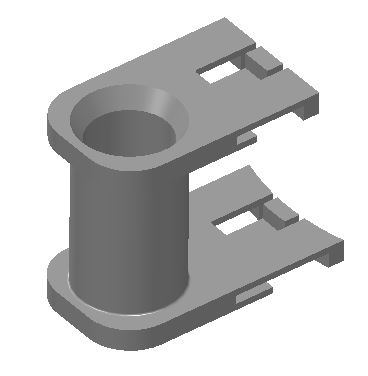
\includegraphics[width = 0.3\textwidth]{Bilder/gleitbuchse_creo}}
					\subfigure[Gefertigte Gleitbuchse\label{gleitbuchse_gefertigt}]{\includegraphics[width = 0.4\textwidth]{Bilder/gleitbuchse_gefertigt}}
				\par\end{centering}
				\caption{Gleitbuchse}
				\label{Gleitbuchse}
			\end{figure}

	Prinzipiell werden zwei Gleitbuchsen gegenüberliegend am Hexacopter montiert, der Copter wird dann auf zwei langen Stangen aufgefädelt und kann sich dadurch nur mehr nach oben und unten bewegen.
	Das soll verhindern, dass der Hexacopter nicht nach links, rechts, vorne oder hinten abdriften kann.
	Beide Buchsen verwenden das spezielle Klammersystem um sie leicht und fest montieren zu können, wie auch die Halterungen für den Ultraschallsensor und die PIXY Cam, werden die Führungen auf die Platte geklippt.
	Die Führungen wurden diesmal auf beide Centerplates befestigt, das bedeutet die obere Klammer musste an die Centerplate angepasst werden.
	Die Centerplates haben komplett verschiedene Ausnehmungen vorgesehen, das erschwerte die Anpassung des Klammersystems um ein Vielfaches.
	Um diese Herausforderung trotzdem lösen zu können, wurden die Platten in Creo ausgemessen und dann auf die Halterungen übertragen.
		 
	Gefertigt wurden beide Teile in dem 3D Drucker der Schule, da die Form der Gleitbuchsen händisch sehr aufwändig zu fertigen werden würden, \bzw es wird sehr viel Gewicht durch diese Fertigungsmethode eingespart.
	Zu beachten war beim Konstruieren wiederum, dass der Drucker grobe Toleranzen hat und diese miteingerechnet werden mussten.

	Die Bohrungen wurden so groß dimensioniert, dass der Hexacopter leicht auf und ab fliegen kann, ohne zu stark zu verkanten.
	Die Phasen bei den Bohrungen oben und unten, lassen den Copter leichter auffädeln, da die Stangen leichter in die Bohrungen führen.

	\subsection{Herausforderungen und Lösungen}

	Das Verkanten zwischen den Buchsen und Stangen war besonders während des Startes ein Problem.
	Der Hexacopter hob zu Beginn etwas  schief ab, das kann man auch nicht mit sehr großen Bohrungen verhindern.
	Es musste manuell mit der Fernsteuerung entgegen dieses Neigens gesteuert werden, damit der Multicopter abheben konnte.
	Nach etwa 5 cm hatte sich der Copter so ausgeglichen, dass nicht mehr entgegen gesteuert werden musste.
	Die Gleitbuchsen haben sich trotzdem sehr bewährt, da der Multicopter, auch wenn er kein Gas mehr gab, nur auf dem Landesgestell landete und so keine Teile beschädigt wurden.

			\newpage

\section{Persönliche Erfahrungen}
